\documentclass{report}
\usepackage[T1]{fontenc} % Fontes T1
\usepackage[utf8]{inputenc} % Input UTF8
\usepackage[backend=biber, style=ieee]{biblatex} % para usar bibliografia
\usepackage{csquotes}
\usepackage[portuguese]{babel} %Usar língua portuguesa
\usepackage{blindtext} % Gerar texto automaticamente
\usepackage[printonlyused]{acronym}
\usepackage{hyperref} % para autoref
\usepackage{graphicx}

\bibliography{bibliografia}


\begin{document}
%%
% Definições
%
\def\titulo{TRABALHO DE APROFUNDAMENTO 2}
\def\data{Abril 2018}
\def\autores{José Pedro Silva, Pedro Silva}
\def\autorescontactos{(89195) jose.silva99@ua.pt, (89228) pedromsilva99@ua.pt}
\def\versao{VERSAO}
\def\departamento{DEPARTAMENTO DE ELETRÓNICA TELECOMUNICAÇÕES E INFORMÁTICA}
\def\empresa{UNIVERSIDADE DE AVEIRO}
\def\logotipo{ua.pdf}
%
%%%%%% CAPA %%%%%%
%
\begin{titlepage}

\begin{center}
%
\vspace*{50mm}
%
{\Huge \titulo}\\ 
%
\vspace{10mm}
%
{\Large \empresa}\\
%
\vspace{10mm}
%
{\LARGE \autores}\\ 
%
\vspace{30mm}
%
\begin{figure}[h]
\center
\includegraphics{\logotipo}
\end{figure}
%
\vspace{30mm}
\end{center}
%
\begin{flushright}
\versao
\end{flushright}
\end{titlepage}

%%  Página de Título %%
\title{%
{\Huge\textbf{\titulo}}\\
{\Large \departamento\\ \empresa}
}
%
\author{%
    \autores \\
    \autorescontactos
}
%
\date{\data}
%
\maketitle

\pagenumbering{roman}

%%%%%% RESUMO %%%%%%
\begin{abstract}
Neste trabalho de aprofundamento 2, foi colocada uma sonda na Universidade de Aveiro que mede os valores instantâneos de temperatura, humidade e vento e é capaz de mandar os dados através de uma rede sem fios. Através do terminal, conseguimos aceder aos valores instantâneos de temperatura, humidade e vento de 10 em 10 segundos.

Podemos comunicar com a sonda através de um socket \ac{tcp},  na porta 8080 do servidor \url{xcoa.av.it.pt}.


O objetivo deste trabalho, era desenvolver um programa na linguagem "Python", que fosse capaz de receber esses valores de temperatura, humidade e vento, realizasse a média dos valores de um certo número de mensagens mandadas pela sonda, e no final devolvesse uma mensagem útil sobre o vestuário que uma pessoa deveria utilizar caso saísse de casa. Um exemplo era mandar uma mensagem a dizer "Leve um casaco" caso a temperatura fosse abaixo dos 15 ºC. 

Na parte final do trabalho era pedido que desenvolvessemos uma forma de cifrar as mensagens em ambos os sentidos.


\end{abstract}

%%%%%% Agradecimentos %%%%%%
% Segundo glisc deveria aparecer após conclusão...
\renewcommand{\abstractname}{Agradecimentos}
\begin{abstract}
Gostaríamos de agradecer ao docente João Paulo Barraca por ter proposto este trabalho.
\end{abstract}


\tableofcontents

%%%%%%%%%%%%%%%%%%%%%%%%%%%%%%%
\clearpage
\pagenumbering{arabic}

%%%%%%%%%%%%%%%%%%%%%%%%%%%%%%%%
\chapter{Introdução}
\label{chap.introducao}

Este documento apresenta o desenvolvimento do Trabalho de Aprofundamento 2.
Neste dosumento explicamos como desenvolvemos o código e qual a sua finalidade.
Este documento \LaTeX tem o capítulo Metodologia, onde enuciamos as funções e a maneira como o programa funciona no terminal e tem uma breve conclusão.


\chapter{Metodologia}
\label{chap.metodologia}
Desenvolvemos alguns programas em Python para tentar reolver o que nos foi pedido.


\section{Desenvolvimento do código em Python}

\subsection{Desenvolvimento do programa Base}
Começamos por desenvolver um programa que, quando corrido, vai buscar os valores emitidos pela sonda.
Esse programa, de nome "ap1base" é um programa simples que conecta-se ao servidor e quando corrido imprime o TOKEN e o "type" : "OK".

\begin{figure}[h]
\center
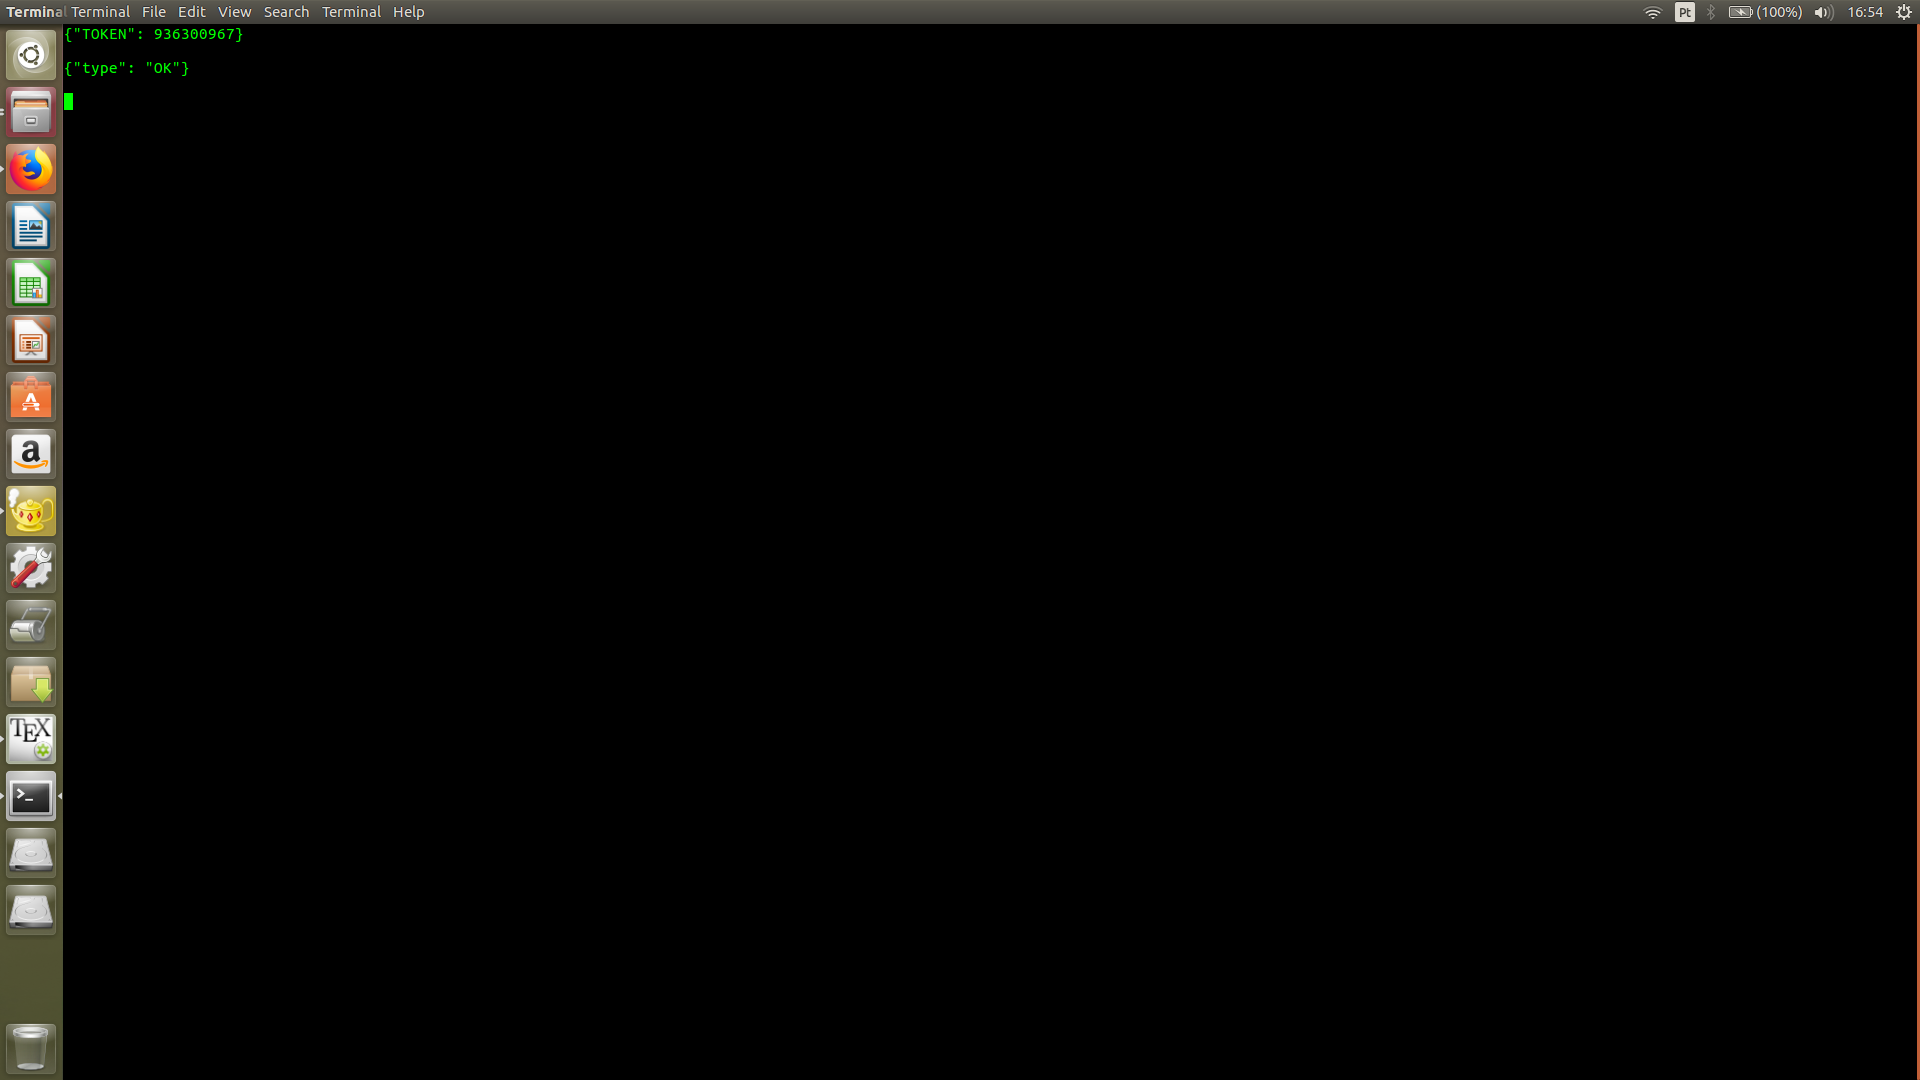
\includegraphics[width=10cm]{Imagens/1.png}
\caption{Abertura do ficheiro ap1base.py no terminal}
\end{figure}

Após uns segundos de espera, começa a receber os valores de tempearatura, humidade e vento da sonda, de 10 em 10 segundos. Enquanto não fecharmos o terminal, vão continuar a ser imprimidos os dados recebidos.

\begin{figure}[h]
\center
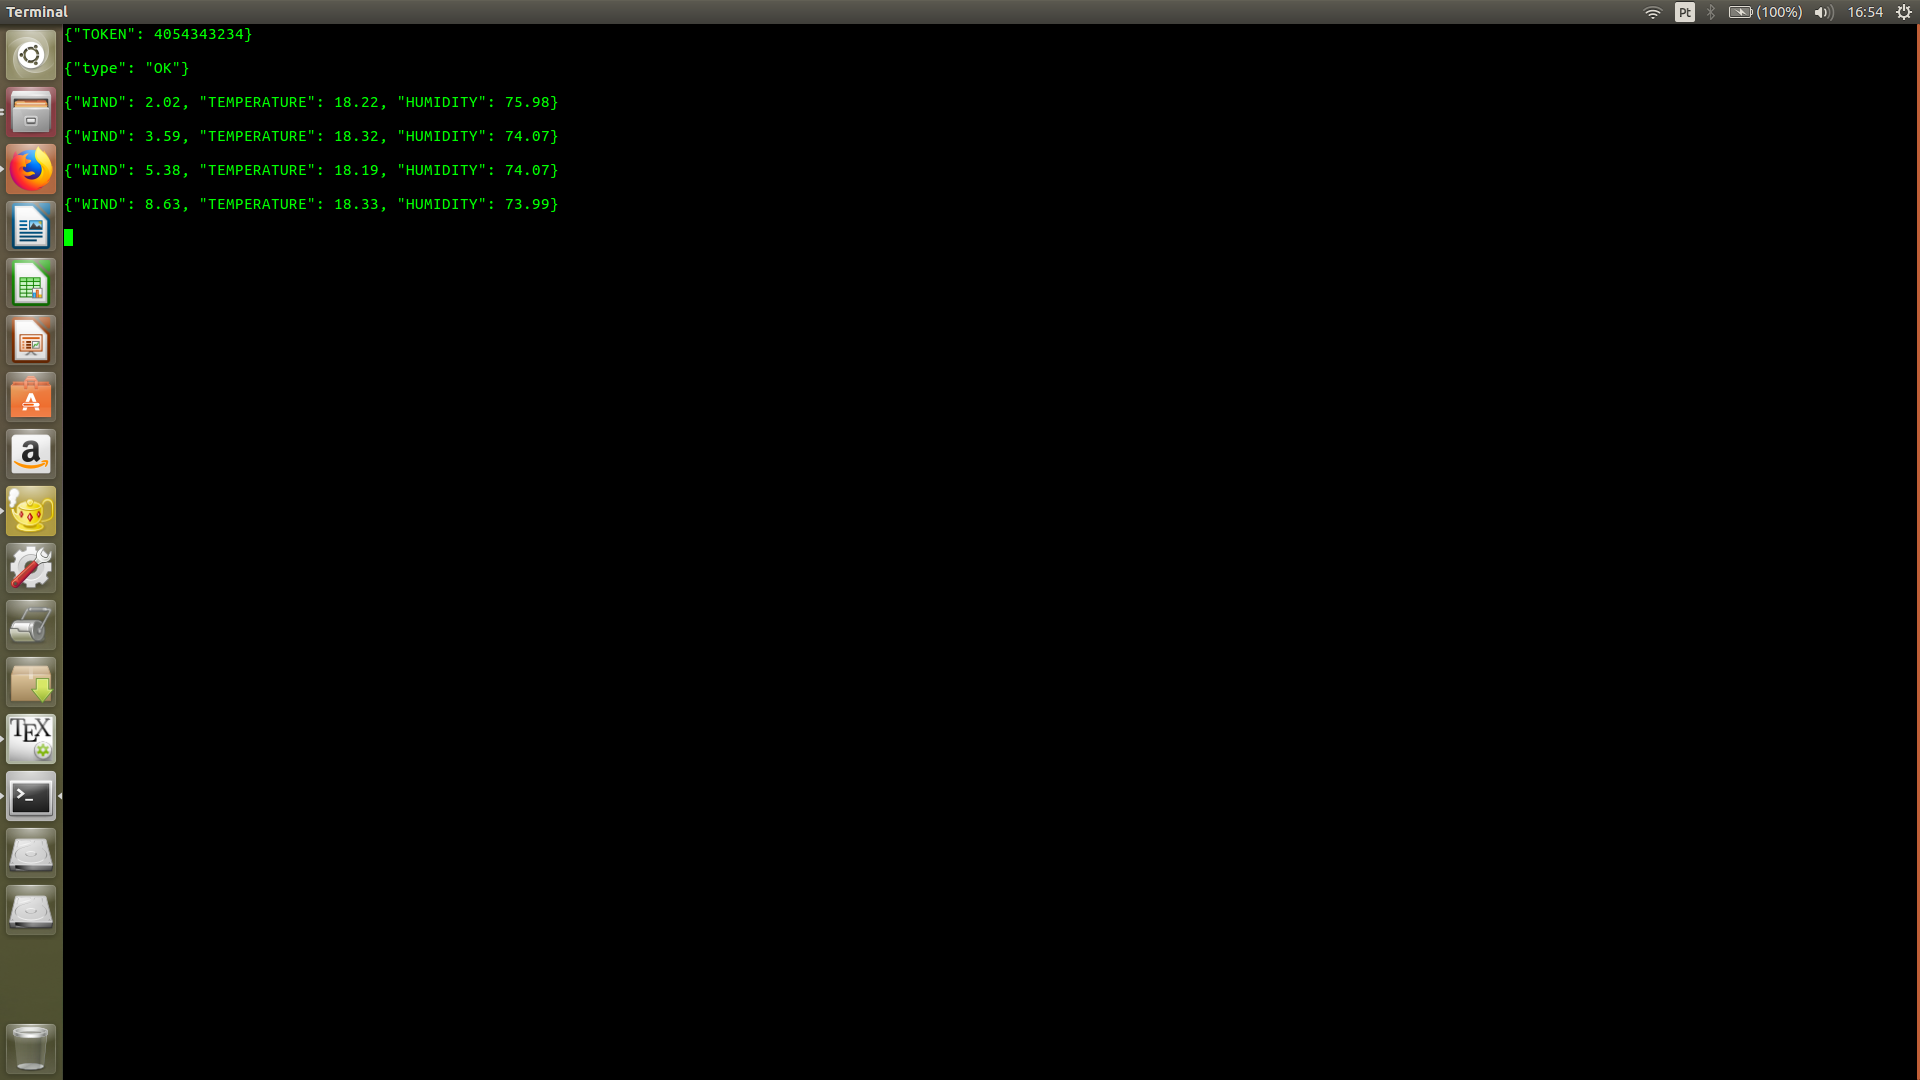
\includegraphics[width=10cm]{Imagens/2.png}
\caption{Programa ap1base.py corrido no terminal e a imprimir as mensagens recebidas pela sonda}
\end{figure}

\subsection{Desenvolvimento do programa AP2}
Este programa, quando corrido faz exatamente o mesmo do ap1base, imprime o TOKEN e o "type" : "OK".

\begin{figure}[h]
\center
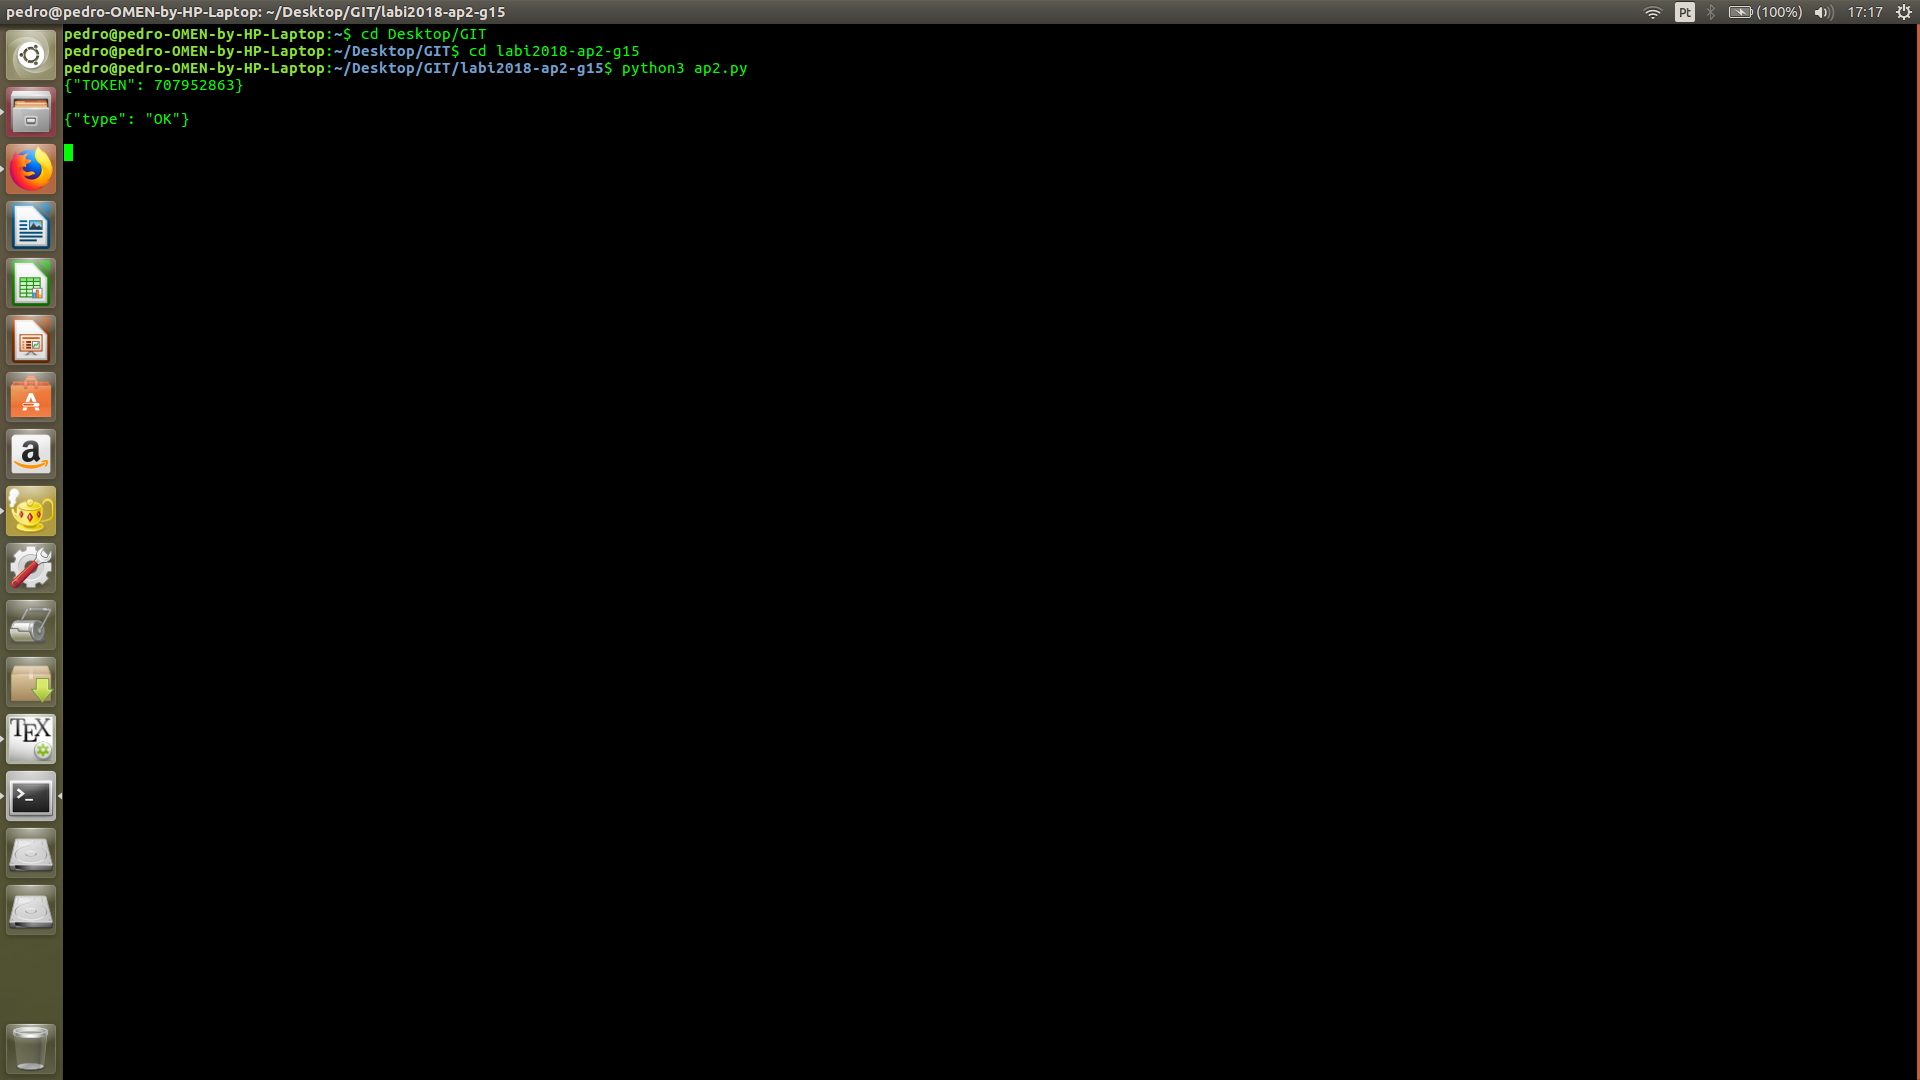
\includegraphics[width=10cm]{Imagens/3.png}
\caption{Abertura do programa ap2.py no terminal}
\end{figure}

A diferença é que quando começa a receber os valores, ao fim de 3 mensagens recebidas e imprimidas no ecrã, apresenta uma frase com dicas sobre vestuário a utilizar.

\begin{figure}[h]
\center
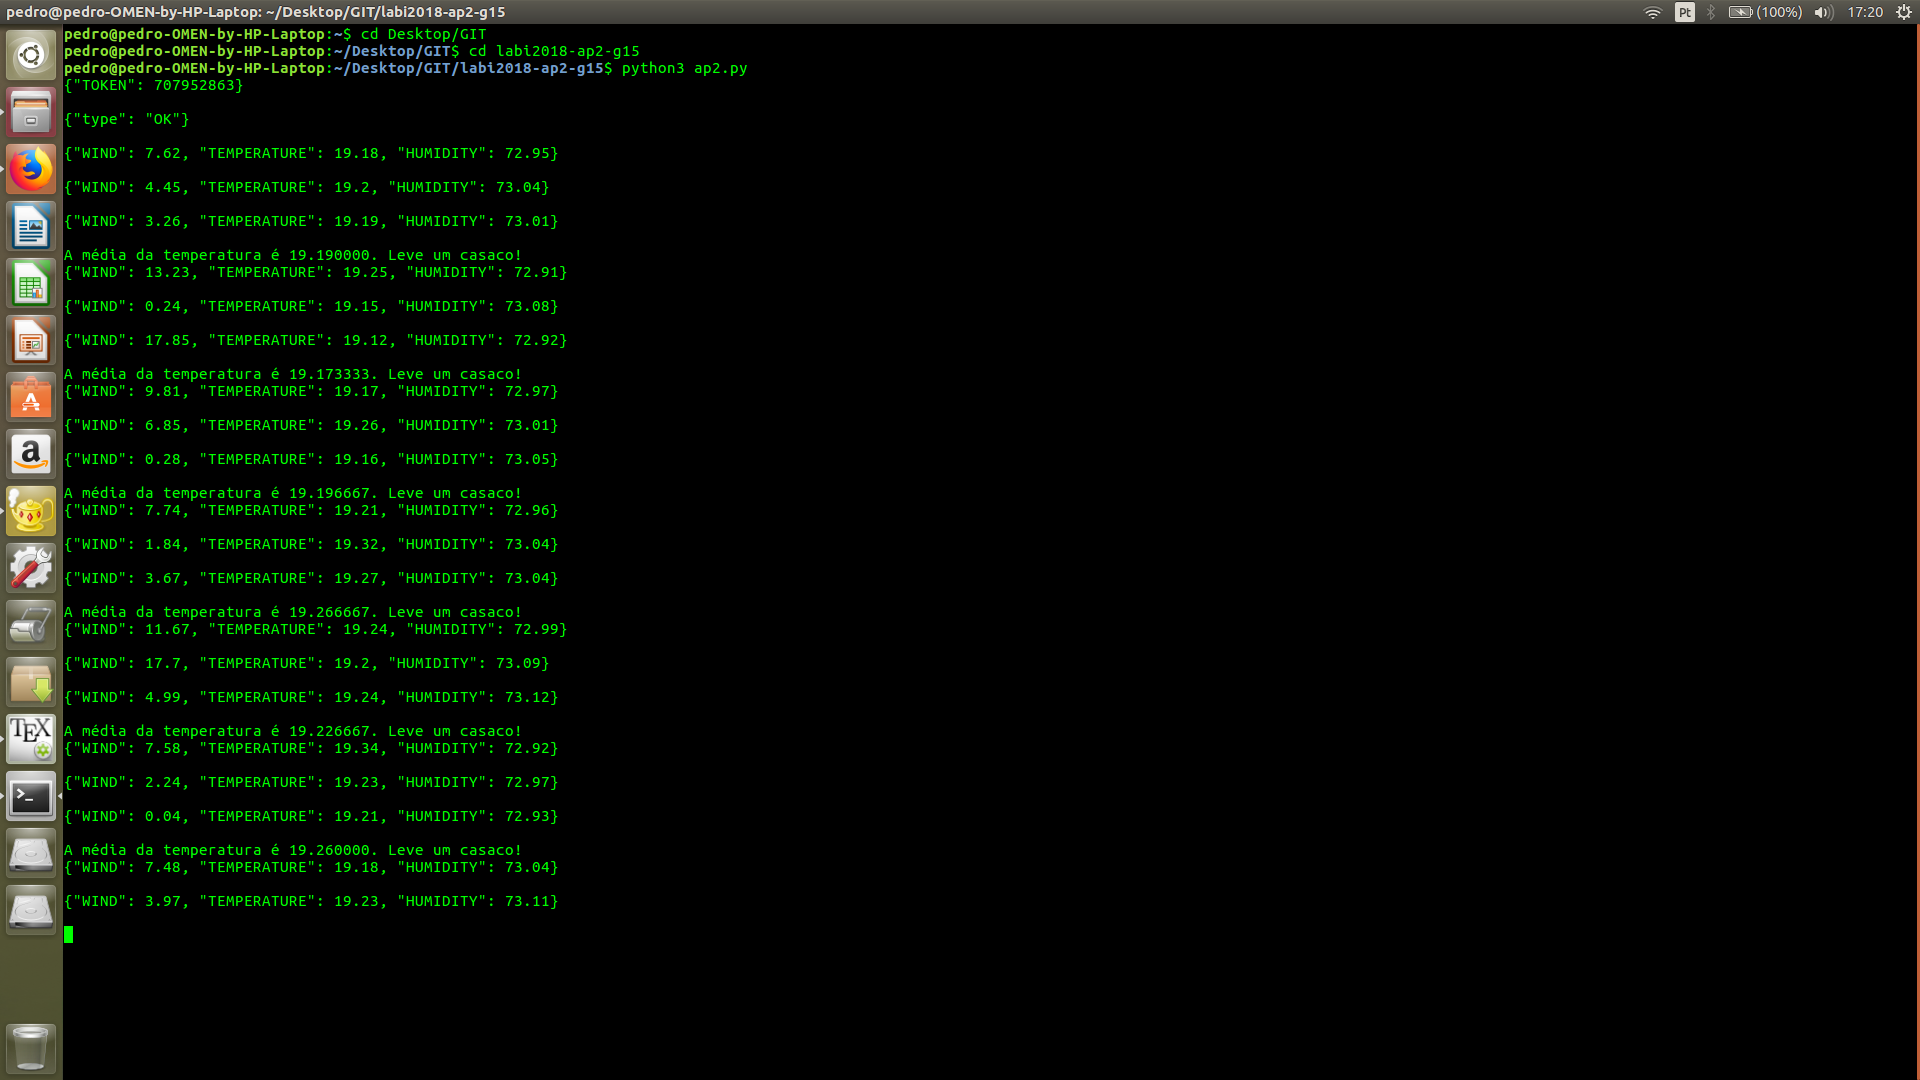
\includegraphics[width=10cm]{Imagens/4.png}
\caption{Programa ap1base.py corrido no terminal e a imprimir as mensagens recebidas pela sonda e mensagens de aviso para quem for sair de casa}
\end{figure}

Este código possui várias funções.
A primeira função, a função "main", que conecta-se ao servidor e imprime os dados recebidos no terminal e guarda-os num ficheiro \ac{csv}. 
O ciclo While chama as outras funções e basicamente é o que comanda as mensagens de aviso imprimidas no terminal. Faz uma contagem das mensagens recebidas da sonda, e importa de outras funções a média da temperatura e a mensagem sobre vestuáio.

A função "weather{\_}info" faz uma contagem das mensagens recebidas, quando a contagem chega a 3, faz a média da temperatura e retorna uma mensagem.

A função "print{\_}csv" faz com que os dados recebidos sejam imprimidos no ficheiro \ac{csv}, por uma determinada ordem, neste caso vento, humidade, temperatura.

A função "f{\_}connect" manda o Connect para o servidor e o Token.


\chapter{Conclusões}
\label{chap.conclusao}
Neste trabalho conseguimos utilizar e melhorar as nossas capacidades em Python, voltamos a trabalhar com Latex após alguns meses sem o fazer, e foi um trabalho em que foi preciso persistência.

A parte da segurança deu-nos bem por vezes, outras vezes deu-nos mal, não conseguimos perceber porquê por isso enviámos essa parte do código em comentário.

Neste trabalho conseguimos fazer várias das coisas pretendidas, mas houve algumas que correram menos bem. 

\chapter*{Contribuições dos autores}
O José Silva trabalhou com o código Python, tendo a atenção do PS. O Pedro Silva fez o relatório e tentou fazer os testes unitários.
Sendo assim, o JS contribuiu em 55\% e o PS em 45\%.

%%%%%%%%%%%%%%%%%%%%%%%%%%%%%%%%%
\chapter*{Acrónimos}
\begin{acronym}
\acro{ua}[UA]{Universidade de Aveiro}
\acro{miect}[MIECT]{Mestrado Integrado em Engenharia de Computadores e Telemática}
\acro{tcp}[TCP]{Transmission Control Protocol}
\acro{csv}[CSV]{Comma Separated Values}
\end{acronym}


%%%%%%%%%%%%%%%%%%%%%%%%%%%%%%%%%
\printbibliography

\end{document}
